% unified_model.tex の和訳（自分の理解用）。内容・数値は英語版と同じ。
% ビルド: lualatex unified_model_ja.tex（2 回）。
\documentclass[11pt,a4paper]{article}
\usepackage{luatexja}
\usepackage[margin=2.2cm]{geometry}
\usepackage{amsmath,amssymb,amsthm}
\usepackage{booktabs,tabularx,array}
\usepackage{enumitem}
\usepackage[hyphens]{url}
\urlstyle{tt}
\usepackage{graphicx}
\graphicspath{{../assets/}}
\setlist{nosep,leftmargin=*}
\newcolumntype{Y}{>{\raggedright\arraybackslash}X}
\theoremstyle{definition}
\newtheorem{proposition}{命題}
\newtheorem{remark}{注意}
\newcommand{\dd}{\,\mathrm{d}}
\newcommand{\D}{\mathrm{D}}
\newcommand{\living}{\textstyle\sum_i s_i\psi_i}
\title{\bfseries 一つの変分原理から導く口腔バイオフィルムの二段モデル\\[2pt]
\large 導出、離散化、検証、最初の結果（和訳）}
\author{西岡佳祐}
\date{作業メモ、2026年10月15日（慶應での続き。修論には入れない）}
\begin{document}
\maketitle

\begin{abstract}
\noindent 修論では、Klempt et al.\ 2024 の成長の場と Klempt et al.\ 2026 の多菌種の点モデルを別々に解き、
Gauss 点でつないでいる。そのため、どの論文も決めていない選択が要る：二つの空隙の関係、点モデルを場に縮めるかどうか、
成長を何で決めるか、点モデルの時間と場の時間の対応。ここではバイオフィルムを二段で表す。相の場 $\phi$（バイオフィルムと外の液体）と、
バイオフィルムの中の、点モデルの組成である。すべての式を、一つのエネルギー、一つの散逸ポテンシャル、一つの拘束から、
Onsager の形の拡張ハミルトン原理で導く。成長は栄養を消費する反応で、生きている量が触媒になる。このモデルは、
場が一様なら点モデルを、組成が相から切り離れた極限では要素の方式 (c) を再現し、Klempt et al.\ 2024 の前線の項なしに
境界が栄養の方へ進む。全体のエネルギーは解に沿って減る。解く離散の式はすべて離散汎関数の自動微分で、実装は点モデルと
丸め誤差まで一致する。較正済みの 5 菌種の点モデルを入れた 3D では、抗菌薬が生きている量、成長、境界の進みを下げ、
全体に効く薬と嫌気性菌に効く薬で違いが出る。組成は局所の栄養で変わる。
\end{abstract}

\section*{やさしい説明}

\paragraph{何が問題だったか。} 修論では、二つのモデルを別々に計算して、あとでつないでいる。場は「バイオフィルムが
どこにどれだけあるか」、点モデルは「中に何の菌がどれだけいて、それぞれ何割生きているか」を決める。つなぐときに、
論文が決めていない選び方が要る。点モデルを場に縮めるか（方式 (a) と (b)）、成長を何で決めるか（方式 (a) と (c)）である。

\paragraph{ここでしたこと。} 二つを最初から一つのモデルとして書き、すべての式を一つの原理から出す。原理は
「系はエネルギーが下がる方へ、摩擦（散逸）で決まる速さで動く」というもの。あとでつなぐ部分がないので、上の選び方が要らなくなる。

\paragraph{分かったこと。}
\begin{enumerate}
\item \emph{空いた所は二種類ある。} バイオフィルムの外の液体と、中の液体は別のもの。混ぜてしまうと、外の液体の中で
  菌が勝手に増える。
\item \emph{成長は栄養を食べる反応。} 生きている菌がこの反応を進めるので、抗菌薬で菌が死ぬと成長が遅くなる。
  生きている菌を「エネルギー」ではなく「反応の速さを決めるもの」として入れることで、抗菌薬がモデルの中で効くようになる。
\item \emph{栄養の方へは自然に広がる。} 栄養の多い側ほどよく育ち、その分、境界がそちらへ押し出される。Klempt et al.\ 2024 は
  これを別の項として足していたが、ここでは成長から出てくる（1D、2D、3D で確認）。
\end{enumerate}

\paragraph{ひとことで。} 修論の方式 (c)（生きている量で成長）は、このモデルを一番簡単にした形である。つまり (c) に理論の裏付けができた。

\paragraph{この先の読み方。} 1〜5 節がモデルと導出、6 節が計算の方法、7 節が確認、8 節が結果、9 節が仮定と未解決。

\section{なぜ二段か}
\label{sec:two}

点モデルを空間にそのまま広げると、各菌種を場 $\phi_i(\mathbf X,t)$ とし、空隙は一つ $\phi_0=1-\sum_i\phi_i$ で、
各点に点モデルのエネルギーを置く形になる。点モデルは障壁のエネルギー $K/[\phi_i^2(1-\phi_i)^2]$ で各 $\phi_i$ を 0 から
離し、増殖は局所である。1D で全部の場を一つの Newton 系として解くと（\path{unified_1d_monolithic.py}）、外の液体が
障壁の床の値から一斉に埋まる（$T^*=1$ でシードから遠い所の量が $0.05$ から $0.43$ に増えた）。つまり、液体の横に
バイオフィルムがある状況を表せない。二つの空隙は別の物理的な対象である：バイオフィルムの外の液体（Klempt et al.\ 2024 の
場が表す）と、中の液体（点モデルの $\phi_0$ が表す）。以下のモデルは両方を残す。

\section{状態}

\begin{center}\small
\begin{tabularx}{\linewidth}{@{}lYl@{}}
\toprule
記号 & 意味 & 出どころ\\
\midrule
$\phi(\mathbf X,t)\in[0,1]$ & バイオフィルムの相：バイオフィルムと外の液体 & Klempt et al.\ 2024\\
$s_i(\mathbf X,t)$, $i=1\dots n$ & バイオフィルムの中の菌種 $i$ の割合 & Klempt et al.\ 2026（そこでの $\phi_i$）\\
$s_0(\mathbf X,t)$ & 中の液体、$\sum_is_i+s_0=1$ & Klempt et al.\ 2026（そこでの $\phi_0$）\\
$\psi_i(\mathbf X,t)$ & 菌種 $i$ の生きた割合 & Klempt et al.\ 2026\\
$\gamma(\mathbf X,t)$ & 組成の拘束の乗数 & Klempt et al.\ 2026\\
$c(\mathbf X,t)$ & 栄養の濃度 & Klempt et al.\ 2024\\
$\alpha(\mathbf X,t)$ & 局所の膨張、$\mathbf F_g=\alpha\mathbf I$、$\alpha(0)=1$ & Klempt et al.\ 2024\\
$\mathbf u(\mathbf X,t)$ & 変位 & Klempt et al.\ 2024\\
\bottomrule
\end{tabularx}
\end{center}
菌種 $i$ の絶対量は $\phi s_i$、生きている量は $\phi\living$。点モデルの $\bar\phi_i=\phi_i\psi_i$ はここでは
$s_i\psi_i$。すべての場は参照配置 $\mathbf X$ の上にある。

\section{エネルギー、散逸、拘束}

$h(\phi)=\phi^2$ をバイオフィルムが組成を担う重みとし、$w=h(\phi)+\varepsilon$ とする。小さい $\varepsilon>0$ は、
重みのない外の液体でも組成の式が壊れないようにするためのもの。

\paragraph{組成。} Klempt et al.\ 2026 の点モデルのエネルギー（バイオフィルム単位量あたり）
\begin{equation}
\Psi_{\rm pm}=\underbrace{K\Big[\sum_iB(s_i)+B(s_0)+\sum_iB(\psi_i)\Big]}_{\Psi_{\rm bar}}
+\underbrace{\frac{\alpha^*}{2}\sum_ib_i\psi_i^2-\frac{c^*}{2}\sum_{ij}A_{ij}\,s_i\psi_i\,s_j\psi_j}_{\Psi_{\rm int}},
\label{eq:pm}
\end{equation}
ここで $B(x)=1/[x^2(1-x)^2]$。障壁の定数 $K=10^{-4}$、種間作用の行列 $A$（較正済み、対称）、栄養の定数 $c^*$、抗菌薬の濃度 $\alpha^*$、
感受性 $b_i$。障壁の項は $s_i,s_0,\psi_i$ を $(0,1)$ の中に保つ。両方とも蓄えられたエネルギーで、重み $w$ を持つ
（注意~\ref{rem:barrier}）。

\paragraph{相、栄養、成長。} Klempt et al.\ 2024 の勾配のエネルギー、$\phi\le1$ を保つ片側の障壁、栄養の理想溶液の
自由エネルギー、育った菌の化学ポテンシャル $\mu_b$ を合わせて、
\begin{equation}
\begin{aligned}
E={}&\frac{\beta}{2}|\nabla\phi|^2+\frac{K_\phi}{(1-\phi)^2}
+\lambda w\,\Psi_{\rm pm}+w\frac{\beta_s}{2}\sum_i|\nabla s_i|^2\\
&+c(\ln c-1)+\mu_b\,\xi+E_{\rm mech},\qquad \xi=\alpha-1 .
\end{aligned}
\label{eq:E}
\end{equation}
$\lambda$ は相に対する組成のエネルギーの尺度、$\beta_s$ はバイオフィルムの中での組成の広がり、
$E_{\rm mech}=\tfrac{\mu}{2}\phi^2(\mathbf I:\mathbf C_e-3)$ は Klempt et al.\ 2024 の力学のエネルギーで、
成長の式には入らない（そこと同じく、成長への効果は小さいとして）。

\paragraph{散逸。} 速さの 2 次。組成は Klempt et al.\ 2026、相は Klempt et al.\ 2024、それに成長の反応の二つの流れ：
\begin{equation}
\D=\frac{\eta_\phi}{2}\dot\phi^2+\lambda w\,\D_{\rm pm}+\frac{\dot\xi^2}{2L}+\frac{|\mathbf j|^2}{2Dc},\qquad
\D_{\rm pm}=\sum_i\Big[\frac{\eta}{2}\dot s_i^2+\frac{\eta}{2}\big(\tfrac{\dd}{\dd t}(s_i\psi_i)\big)^2\Big]+\frac12\dot s_0^2 ,
\label{eq:D}
\end{equation}
$\mathbf j$ は栄養の流束、$L$ は成長の反応の移動度。生きている量がその触媒で、
\begin{equation}
L=L_0\,\phi\living ,
\label{eq:L}
\end{equation}
溶菌や抗菌薬は移動度を通して成長を下げ、$\psi_i$ には力を及ぼさない（注意~\ref{rem:catalyst}）。

\paragraph{拘束。} 乗数の場による組成の拘束 $\lambda w\gamma(\sum_is_i+s_0-1)$ と、栄養 $Y$ 単位を成長 1 単位に変える
反応の収支
\begin{equation}
\dot c+Y\dot\xi+\nabla\!\cdot\mathbf j=0 .
\label{eq:balance}
\end{equation}

\section{原理と発展方程式}

状態 $q=\{\phi,s_i,s_0,\psi_i,\gamma\}$ に対し、Junker と Balzani の拡張ハミルトン原理（Klempt et al.\ 2024 が使う形）は
\begin{equation}
\delta_q\int_\Omega E\dd V+\int_\Omega\frac{\partial\D}{\partial\dot q}\,\delta q\dd V=0
\qquad\forall\,\delta q,
\label{eq:principle}
\end{equation}
境界で $\mathbf n\cdot\nabla\phi=\mathbf n\cdot\nabla s_i=0$。散逸は速さについてだけ変分する。反応と流束については
Onsager の形で、$\dot\xi$ と $\mathbf j$ は収支 \eqref{eq:balance} のもとで Rayleigh 汎関数
$\frac{\dd}{\dd t}\int E+\int\D$ を最小にする。

\paragraph{組成}（各式を $\lambda w>0$ で割った形）：
\begin{align}
KB'(s_i)+\gamma+\eta(1+\psi_i^2)\dot s_i+\eta s_i\psi_i\dot\psi_i-c^*\psi_i\sum_jA_{ij}s_j\psi_j
-\frac{\beta_s}{\lambda w}\nabla\!\cdot(w\nabla s_i)&=0,\label{eq:s}\\
KB'(s_0)+\gamma+\dot s_0&=0,\\
KB'(\psi_i)+\alpha^*b_i\psi_i+\eta s_i\psi_i\dot s_i+\eta s_i^2\dot\psi_i-c^*s_i\sum_jA_{ij}s_j\psi_j&=0,\label{eq:psi}\\
\textstyle\sum_is_i+s_0-1&=0 .
\end{align}
勾配の項を除けば、各点で自分の時間で進む Klempt et al.\ 2026 の点モデルそのもの。

\paragraph{相：}
\begin{equation}
\eta_\phi\dot\phi-\beta\nabla^2\phi+\frac{2K_\phi}{(1-\phi)^3}
+\lambda h'(\phi)\Psi_{\rm pm}+h'(\phi)\frac{\beta_s}{2}\sum_i|\nabla s_i|^2=0 .
\label{eq:phi}
\end{equation}
組成は $\lambda h'(\phi)\Psi_{\rm pm}$ を通して相に働く。組成のエネルギーが低い所（強い有利な種間作用）では
バイオフィルムが増えやすく、高い所（抗菌薬、$\alpha^*b_i\psi_i^2/2$）では減りやすい。$h'(0)=0$ なので、
バイオフィルムのない所では組成は力を及ぼさない。

\paragraph{成長と栄養。} $\mu_c=\partial_cE=\ln c$ として、\eqref{eq:balance} のもとでの Rayleigh 汎関数から
\begin{equation}
\dot\xi=L\,(Y\ln c-\mu_b),\qquad \mathbf j=-D\nabla c,\qquad
\dot c=D\nabla^2c-Y\dot\xi ,
\label{eq:growth}
\end{equation}
補給の境界で $c=1$、ほかでは $\mathbf n\cdot\nabla c=0$。$\mu_b=Y\ln c_{\rm stop}$ と書くと、$c$ が $c_{\rm stop}$ まで
下がった所で成長が止まる。運動学は Klempt et al.\ 2024 の $\mathbf F=\mathbf F_e\mathbf F_g$、$\mathbf F_g=\alpha\mathbf I$。

\paragraph{力学。} Klempt et al.\ 2024 の剛性 $(\phi^2+f)E_{\rm bio}$ による仮想仕事の原理。変更なし。

\begin{remark}[障壁の項]\label{rem:barrier}
一段の点モデルでは $\Psi_{\rm bar}$ の微分しか効かない。バイオフィルムの量で重みをつけると、その値も
$\lambda h'(\phi)\Psi_{\rm bar}$ として相に働く。較正の開始状態（$\psi_i=0.999$）ではこの値は約 $500$ で、種間作用の約 $8$
よりずっと大きい。最初の過渡（$\psi_i\approx0.9$）のあとは $0.1$ 以下になる。二つの代案を試した。障壁の重みを固定する
（正則化した拘束）形と、重みを定数にする形で、どちらも $\alpha$ を約 $6\,\%$ 変え、前者は厳密なエネルギー不等式を壊す。
文字どおりの形、つまり障壁を重み $w$ つきの蓄えられたエネルギーとして扱う形を採る。Klempt et al.\ 2026 がそう書いていて、
命題~\ref{prop:energy} が厳密に成り立つからである。
\end{remark}

\begin{remark}[成長のエネルギーか、成長の反応か]\label{rem:catalyst}
最初の版は、成長をエネルギー $-k_\alpha(\alpha-1)\phi\living$ で駆動した。これは $\dot\alpha=k_\alpha\phi\living$ を
直接与える。しかしその $\psi_i$ による微分は、成長した所で菌を生かし続ける力になり、成長が大きいと抗菌薬に勝つ
（$k_\alpha=8$ では抗菌薬で成長が $0.7\,\%$ しか下がらなかった）。反応の形 \eqref{eq:growth}--\eqref{eq:L} は
生きている量を移動度に入れる。触媒は速さを変え、エネルギーは変えない、という本来の場所である。$k_\alpha$ を意味のある量
（$L_0$、$Y$、$c_{\rm stop}$）に置き換え、エネルギー不等式に栄養を含める形にもなる。
\end{remark}

\section{性質}

\begin{proposition}[エネルギー不等式]\label{prop:energy}
$E$ が時間に陽に依らず、境界が閉じている（$\mathbf n\cdot\mathbf j=0$）とする。\eqref{eq:s}--\eqref{eq:growth} の解に沿って
\[\frac{\dd}{\dd t}\int_\Omega E\dd V=-\int_\Omega\Big[2\lambda w\D_{\rm pm}+\eta_\phi\dot\phi^2
+\frac{\dot\xi^2}{L}+\frac{|\mathbf j|^2}{Dc}\Big]\dd V\le0 .\]
\end{proposition}
\begin{proof}
\eqref{eq:principle} の各停留条件にその速さを掛け、積分して足す。勾配の項は部分積分で勾配のエネルギーの時間微分になる
（境界項は無流束の条件で消える）。拘束の項は $\lambda w\gamma\frac{\dd}{\dd t}(\sum_is_i+s_0)=0$。$\D_{\rm pm}$ と
$\dot\phi^2$ は速さの 2 次なので、速さと散逸の力の積は散逸の 2 倍になる。反応については、部分積分のあと
$\partial_cE\,\dot c+\mu_b\dot\xi=\mu_c(-Y\dot\xi-\nabla\!\cdot\mathbf j)+\mu_b\dot\xi
=-(Y\mu_c-\mu_b)\dot\xi+\mathbf j\cdot\nabla\mu_c$ で、\eqref{eq:growth} から $Y\mu_c-\mu_b=\dot\xi/L$、
$\nabla\mu_c=-\mathbf j/(Dc)$。
\end{proof}

\begin{remark}
補給の境界（$c=1$）と抗菌薬の切り替え（$\alpha^*$ が時間で変わる）は外からの入力である。前者は栄養のエネルギーの流入、
後者は $\int\lambda w\,\tfrac12\dot\alpha^*\sum_ib_i\psi_i^2$ を足す。計算では、離散のエネルギーが増えるのはこの二つだけである。
\end{remark}

\paragraph{極限。}
\begin{enumerate}
\item 一様な場、$\beta_s=0$：各点の組成は、自分の時間で進む Klempt et al.\ 2026 の点モデル。較正した $A$、$c^*$、
  較正の時間の対応がそのまま使える。
\item $\lambda\to0$、$\beta_s=0$：組成は相から切り離れ、バイオフィルムのある所で、要素の独立した点モデル（方式 (b)）として動く。
  成長 $\dot\alpha=L_0\phi\living\,(Y\ln c-\mu_b)$ は要素の方式 (c)、$\dot\alpha=\kappa\,\phi_{3D}\sum_i\bar\phi_i$ で、
  $\kappa=L_0(Y\ln c-\mu_b)$。つまり方式 (c) はこのモデルの切り離れた極限で、縮めずに動かすその点モデルが整合する形である。
  その $\phi_0$ は中の液体 $s_0$。
\item 方式 (a)（点モデルを $\sum_i\phi_i=\phi_{3D}$ に縮める）は中と外の液体を同一視する。このモデルの極限ではない。
\item 1 種、$\psi\equiv1$、$c$ 一定：$\dot\alpha=L_0\phi\,(Y\ln c-\mu_b)$ は Klempt et al.\ 2024 の Eq.~36 で、
  $k_\alpha=L_0(Y\ln c-\mu_b)$。
\end{enumerate}

\begin{proposition}[前線は運動学で動く]\label{prop:front}
基板の上のバイオフィルムの層が、基板に垂直な方向にだけ伸びるとする。現在の配置での境界は
$x(t)=\int_0^{X_e}\alpha^3(X',t)\dd X'$ にある。$X_e$ は参照配置での境界。境界は成長の積分の速さで進む。
Wanner と Gujer のモデルで前線の速さが生産の積分であるのと同じである。
\end{proposition}
\begin{proof}
$\mathbf F_g=\alpha\mathbf I$ から体積比は $J=\alpha^3$。垂直方向にだけ伸びるなら、その方向の伸びが $J$ なので
$\dd x=\alpha^3\dd X$。
\end{proof}
Klempt et al.\ 2024 は相の式に前線の項 $h^*_\phi$ を足している。これはポテンシャルから導かれていない（彼らの Remark~1）。
このモデルでは境界は成長そのもので動くので、前線の項を足すと同じ成長を二重に数えることになる。2D と 3D では、
方向は栄養から決まる。$c$ が高い所ほど成長が大きく、境界がより進む（\ref{sec:results} 節）。

\section{離散化と解き方}

空間は 1 次元（無流束のために端を折り返した節点、節点求積）、時間は後退 Euler。$U^n$ から $U$ への 1 刻みで離散汎関数
\[\Pi(U)=E_h(U)+\Delta t\,\D_h\Big(\frac{U-U^n}{\Delta t};\,U\Big)+C_h(U)\]
を書き（エネルギー、新しい状態で重みと係数を固定した散逸、拘束）、残差をその自動微分（JAX）$R(U)=\partial_U\Pi$ とする
（行は点モデルの形に合わせて尺度を直す）。したがって離散の式は構成上、離散の Euler--Lagrange 方程式で、手で打った式はない
（\path{unified_two_level_1d.py}、\path{unified_two_level_fuel_1d.py}）。Jacobian は $R$ の自動微分（固定した重みを通した依存も含む）。
Newton 法に、$s,\psi\in(0,1)$、$0<\phi<1$、$c>0$ を保つ減衰をつけ、$|R|_\infty<10^{-8}$ まで解く。収束しない刻みは再帰的に半分にする。

2D と 3D の前線の確認（\path{fuel_front_2d.py}、\path{fuel_front_3d.py}、\path{fuel_front_3d_species.py}）は切り離れた極限を使う。
規則格子の上で栄養と成長 \eqref{eq:growth} を、バイオフィルムの各節点の点モデル（毎刻み減衰 Newton で $|Q|<10^{-10}$ まで）と
ともに解き、$T^*=1$ で一度だけ力学を解く。微小ひずみ、線形弾性、成長の固有ひずみ $(\alpha-1)\mathbf I$、
剛性 $(\phi^2+f)E_{\rm bio}$、$\nu=0.3$、基板固定。これは運動学の確認で、本来のモデルは Klempt et al.\ 2024 の力学を使う。

\section{検証}

\begin{center}\small
\begin{tabularx}{\linewidth}{@{}Yp{3.4cm}p{4.3cm}@{}}
\toprule
確認 & 結果 & ファイル\\
\midrule
残差 $=$ 汎関数の勾配を、独立に手で書いた残差と行ごとに比較 & 組成の行は丸め誤差まで一致。相の行は、手書き版が近似した項のぶん違う
& \path{unified_two_level_variational_check.py}\\
1 節点、結合なし：組成の行がリポジトリの点モデルの残差（\path{core_hamilton_1d.residual}）に等しい & 全行、丸め誤差まで & 同じ\\
一様な場、$\beta_s>0$、成長なし：各節点が収束まで解いた点モデルに等しい & $8.9\times10^{-11}$（二段）、$1.6\times10^{-13}$（一段）
& \path{unified_two_level_1d.py}、\path{unified_1d_monolithic.py}\\
離散のエネルギー、全刻み、閉じた系 & すべての刻みで減少。増えるのは抗菌薬の切り替えだけ & \path{unified_two_level_1d.py}（二段）、
\path{unified_two_level_fuel_1d.py}（栄養つき）\\
Newton & 全刻みで $|R|_\infty<10^{-8}$、最大 31 回 & \path{unified_two_level_1d.py}\\
時間刻み、1D & 60 刻みと 120 刻み：$\alpha-1$ の違い $0.7\,\%$ & 同じ\\
メッシュ、3D（組成ひとまとめ） & $16^3$、$24^3$、$32^3$：境界の変位の違い $3\,\%$ 以内 & \path{fuel_front_3d.py}\\
メッシュ、3D（5 菌種） & $16^3$ と $24^3$：$8\,\%$ 以内（$c^*$ 一定）、$9\,\%$ 以内（局所栄養） & \path{fuel_front_3d_species.py}\\
3D の中の点モデル & 全刻みで残差 $\le4.5\times10^{-13}$ & 同じ\\
\bottomrule
\end{tabularx}
\end{center}

\section{結果}
\label{sec:results}

すべて Heine et al.\ の常在・流れの条件（CH）で較正した点モデルを使う。較正の Day-1 の状態を中の液体 $s_0=0.1$ に置いて始め、
較正の時間の対応（点モデルの時間で $T^*$ あたり $0.2375$、$T^*=1$ が Day~21）。抗菌薬のパラメータは仮定：全菌種で同じ感受性
（$b_i=1$、$\alpha^*=0.65$）、または嫌気性菌（\textit{V.~dispar}、\textit{F.~nucleatum}、\textit{P.~gingivalis}）が 10 倍敏感
（$\alpha^*=0.32$）。$T^*=0.5$ から入れる。

\paragraph{1D、成長を反応にした二段モデル。} シード $\phi=0.9$（$x\le0.25$）、外の液体 $10^{-4}$、栄養は $x=1$ から補給。
$\lambda=1$、$\beta=\beta_s=0.02$、$L_0=0.7$、$Y=1$、$c_{\rm stop}=0.1$、$D=1$。
\begin{center}\small
\begin{tabular}{@{}lcccc@{}}
\toprule
& $\alpha-1$（$x=0$、$0.2$） & $c$（$x=0$、$0.25$） & $\phi(0)$ & 基板の生きた割合\\
\midrule
抗菌薬なし & $0.137$、$0.118$ & $0.938$、$0.949$ & $0.77$ & $0.53$\\
$T^*=0.5$ から抗菌薬（全菌種） & $0.116$、$0.102$ & $0.951$、$0.959$ & $0.67$ & $0.31$\\
\bottomrule
\end{tabular}
\end{center}
抗菌薬で成長は $15\,\%$ 下がり、生きた割合は $0.53$ から $0.31$ に、相そのものも下がり、栄養が余る。閉じた系では離散の
全体のエネルギーがすべての刻みで減る（最大の変化 $-8.6\times10^{-3}$）。現在の配置での境界（命題~\ref{prop:front}、$L_0=3$）は、
栄養が豊か（$c_{\rm stop}=0.1$）なら $T^*=1$ までに $0.25$ から $0.80$ へ、乏しい（$c_{\rm stop}=0.5$）なら $0.35$ へ、
$T^*=0.5$ からの抗菌薬では $0.62$ へ進む。

\paragraph{1D、感度。} 反応のかわりに注意~\ref{rem:catalyst} の成長のエネルギーを使い（基準 $k_\alpha=2$）、
パラメータを 1 つずつ変える。$T^*=1$。
\begin{center}\footnotesize
\begin{tabular}{@{}llcccc@{}}
\toprule
パラメータ & 値 & $\alpha-1$（$x=0$） & $\phi$（$x=0$、$0.3$、$1$） & 生きた割合 & 抗菌薬：$\Delta(\alpha-1)$、$\Delta\phi(0)$\\
\midrule
$\lambda$ & $0.3$ & $0.236$ & $0.90$、$0.31$、$10^{-4}$ & $0.79$ & $-5\,\%$、$-0.04$\\
 & $1$（基準） & $0.183$ & $0.81$、$0.28$、$10^{-4}$ & $0.59$ & $-11\,\%$、$-0.12$\\
 & $3$ & $0.125$ & $0.60$、$0.21$、$10^{-4}$ & $0.54$ & $-18\,\%$、$-0.22$\\
$k_\alpha$ & $0.5$ & $0.043$ & $0.77$、$0.27$、$10^{-4}$ & $0.52$ & $-16\,\%$、$-0.11$\\
 & $8$ & $1.339$ & $0.99$、$0.68$、$10^{-4}$ & $0.94$ & $-1\,\%$、$0.00$\\
$\beta$ & $0.005$ & $0.183$ & $0.81$、$0.17$、$10^{-4}$ & $0.59$ & $-12\,\%$、$-0.12$\\
 & $0.08$ & $0.171$ & $0.67$、$0.34$、$3\times10^{-4}$ & $0.59$ & $-10\,\%$、$-0.10$\\
$\beta_s$ & $0.005$、$0.08$ & $0.183$ & $0.81$、$0.28$、$10^{-4}$ & $0.59$ & $-11\,\%$、$-0.12$\\
\bottomrule
\end{tabular}
\end{center}
外の液体はどの場合も空のまま。$\lambda$ は抗菌薬が成長と相にどれだけ効くかを決め、$\beta$ は広がり方を決め、
$\beta_s$ は組成が一様なシードでは効かない。$k_\alpha=8$ の行は、反応の形に変える理由になった成長エネルギーの欠陥を示す
（注意~\ref{rem:catalyst}）。

\paragraph{2D と 3D、前線の方向。} 基板の上の半円（2D）または半球（3D）、半径 $0.25$。栄養は $x=1$ の面からだけ補給し、
液体は $c_{\rm stop}$ から始める。組成はひとまとめ（生きた割合 $0.5$）。$L_0=2$、$D=0.2$。
\begin{center}\small
\begin{tabular}{@{}llccc@{}}
\toprule
& メッシュ & 栄養側 & 反対側 & 比\\
\midrule
2D、$30^\circ$ & $48^2$、$D=0.2$ & $0.0180$ & $0.0053$ & $3.4$\\
2D、$30^\circ$ & $48^2$、$D=1$ & $0.0532$ & $0.0377$ & $1.4$\\
3D、仰角 $30^\circ$ & $16^3$ & $0.0190$ & $0.0049$ & $3.9$\\
3D、仰角 $30^\circ$ & $24^3$ & $0.0206$ & $0.0050$ & $4.1$\\
3D、仰角 $30^\circ$ & $32^3$ & $0.0213$ & $0.0051$ & $4.2$\\
\bottomrule
\end{tabular}
\end{center}
$T^*=1$ での境界の外向きの変位。境界は成長の運動学だけで栄養の方へ進み、補給が遅いほど偏る。

\begin{center}
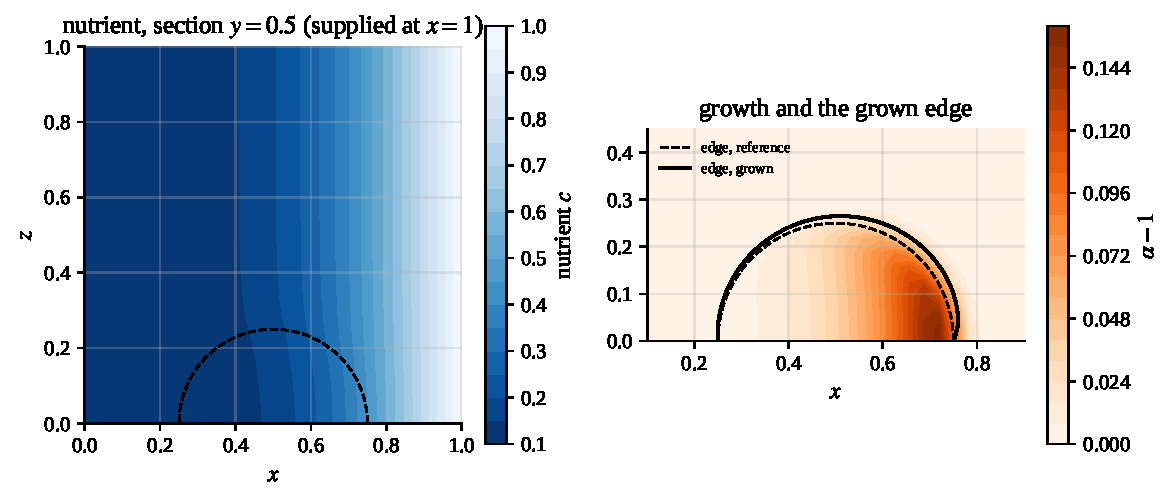
\includegraphics[width=0.85\linewidth]{fig_fuel_front_3d.pdf}\\
{\small 3D、$y=0.5$ の断面：栄養（左）と、成長と育った境界（右）。$24^3$。}
\end{center}

\paragraph{3D、5 菌種の点モデル。} 上と同じ設定で、バイオフィルムの各節点に較正済みの点モデルを置く。$24^3$、$D=0.2$、$L_0=2$。
\begin{center}\small
\begin{tabularx}{\linewidth}{@{}Ycccc@{}}
\toprule
& 中心の生きた割合 & $\alpha-1$、栄養側 / 反対側 & 境界 $30^\circ$、栄養側 / 反対側\\
\midrule
抗菌薬なし & $0.518$ & $0.116$ / $0.005$ & $0.0186$ / $0.0047$\\
抗菌薬、全菌種 & $0.281$ & $0.086$ / $0.003$ & $0.0137$ / $0.0033$\\
抗菌薬、嫌気性菌 & $0.092$ & $0.057$ / $0.002$ & $0.0090$ / $0.0019$\\
\midrule
\multicolumn{4}{@{}l}{点モデルが局所の栄養を見る場合（種間作用 $c^*c(\mathbf x)/c_{\rm ref}$、$c_{\rm ref}=1$）：}\\
抗菌薬なし & $0.507$ & $0.135$ / $0.005$ & $0.0216$ / $0.0053$\\
抗菌薬、全菌種 & $0.332$ & $0.111$ / $0.004$ & $0.0176$ / $0.0043$\\
抗菌薬、嫌気性菌 & $0.354$ & $0.109$ / $0.004$ & $0.0174$ / $0.0044$\\
\bottomrule
\end{tabularx}
\end{center}
局所の栄養を入れると組成が空間で変わる。栄養側（$D=1$ で $c=0.67$）では \textit{V.~dispar} が $0.19$ に増え、
生きた割合が $0.37$ に下がる。反対側（$c=0.38$）では $0.16$ と $0.44$。栄養の乏しい所では種間作用が弱く、
生き残る菌が多い。抗菌薬による境界の変位の減りは、種間作用が一様なとき全菌種 $26\,\%$、嫌気性菌 $52\,\%$、
局所の栄養では $19\,\%$ と $20\,\%$。ここでは場と点モデルが同じ時間を使う（どちらも $T^*=1$ が Day~21）。
最初の 3D の計算では点モデルが Day~5 ごろまでしか進んでおらず、抗菌薬の効きがずっと小さく出ていた。

\begin{center}
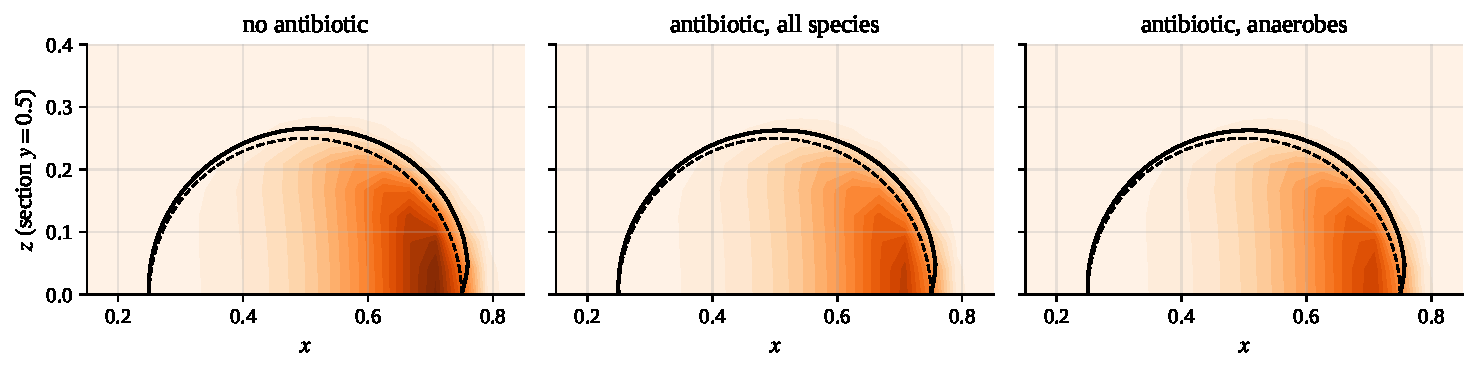
\includegraphics[width=\linewidth]{fig_fuel_front_3d_species_local.pdf}\\
{\small 3D、5 菌種、局所栄養、$y=0.5$ の断面：$\alpha-1$ と育った境界。抗菌薬なし、全体に効く薬、嫌気性菌に効く薬。}
\end{center}

\section{有限要素での実装}
\label{sec:fem}

モデルを Abaqus のユーザー要素として書いた（\path{p3/uel/unified_uel.f90}）。8 節点六面体で、節点に変位、$\phi$、$c$
（Abaqus の自由度 1--3、11、12）、$2\times2\times2$ の Gauss 点に組成、成長 $\xi=\alpha-1$、開始の印を持つ。
相と栄養の式と成長 \eqref{eq:growth} は陰的に解き、組成は増分ごとに一度、$\phi$ が $\phi_{\min}=0.05$ を超えた Gauss 点で
Klempt et al.\ 2026 の点モデルで進める（増分の初めの栄養を使う交互解法）。力学は有限ひずみで、
$\mathbf F=\mathbf F_e\mathbf F_g$、$\mathbf F_g=\alpha\mathbf I$、参照体積あたりのエネルギーは
\[W=\alpha^3(\phi^2+f)\Big[\frac{\mu}{2}\big(J_e^{-2/3}\,\mathbf I:\mathbf C_e-3\big)+\frac K2(J_e-1)^2\Big].\]
Klempt et al.\ 2024（Eq.~20）の力学の項で、非圧縮の拘束を体積のペナルティで置き換えた。微小ひずみも選べる。
接線は式で書いた。抗菌薬は要素の 2 つの値で、決めた時刻に入れられる。場と点モデルは同じ時間を使う（どちらも $T^*=1$ が Day~21）。

クラウドには Abaqus がないので、Abaqus の引数どおりに要素の入口を呼んで確かめた（\path{p3/uel/emulate_abaqus.py}）。
Abaqus の中での実行が次の段階。

\begin{center}\small
\begin{tabularx}{\linewidth}{@{}Yp{5.4cm}@{}}
\toprule
確認 & 結果\\
\midrule
1 要素、一様な場：Gauss 点の組成と、収束まで解いた点モデル & $7.8\times10^{-16}$\\
1D の柱、20 と 40 要素、1D の差分のモデル（\ref{sec:results} 節）と & $\alpha-1$ $0.1371$ / $0.1370$（1D：$0.137$）、
$\phi(0)$ $0.776$ / $0.772$（$0.77$）、$c(0)$ $0.936$ / $0.938$（$0.938$）\\
同じ増分で繰り返し呼ぶ（Abaqus の反復と同じ） & 残差、接線、状態が完全に同じ\\
式で書いた接線と中心差分 & $8.7\times10^{-10}$（全行）、$7.2\times10^{-11}$（力学、変位勾配 $0.3$ 程度）\\
自由な成長 $\mathbf u=(\alpha-1)\mathbf X$ & 力学の残差 $2\times10^{-21}$\\
3D のシード、$16^3$、微小ひずみ、差分の 3D モデル（$\lambda=0$）と & 中心の $\phi$ $0.778$ / $0.779$、境界 $0.0135$ / $0.0126$、
抗菌薬 $-23\,\%$ / $-24\,\%$\\
有限ひずみと微小ひずみ、$8^3$ & 境界 $0.0141$ と $0.0143$（$\alpha-1\approx0.07$）\\
$\nu=0.49$、3D のシード、vM 平均（$8^3$ / $16^3$） & 全積分 $0.0232$ / $0.0201$、平均膨張 $0.0134$ / $0.0163$（$\nu=0.3$：$0.0130$ / $0.0144$）\\
\bottomrule
\end{tabularx}
\end{center}

\paragraph{3D、組成が相に効く場合（$\lambda=1$）。} 差分、$16^3$、点モデルは全節点・全刻みで収束。点モデルのエネルギーの
絶対値は較正で決まっていない（点モデルには微分しか効かない）。$\lambda>0$ ではその値が相を押し下げ、基準なしでは抗菌薬が
なくてもバイオフィルムが $16\,\%$ 縮む。基準 $\Psi_{\rm ref}=0.32$（抗菌薬なしの点モデルのエネルギーの時間平均）を入れると、
抗菌薬なしは $\lambda=0$ に近く、抗菌薬でバイオフィルムそのものが縮む。
\begin{center}\small
\begin{tabularx}{\linewidth}{@{}Yccc@{}}
\toprule
& バイオフィルムの体積（参照配置） & 中心の $\phi$ & 境界 $30^\circ$\\
\midrule
$\lambda=0$、抗菌薬なし & $0.0361$ & $0.78$ & $0.0126$\\
$\lambda=0$、抗菌薬 & $0.0361$ & $0.78$ & $0.0096$\\
$\lambda=1$、$\Psi_{\rm ref}=0.32$、抗菌薬なし & $0.0351$ & $0.78$ & $0.0115$\\
$\lambda=1$、$\Psi_{\rm ref}=0.32$、抗菌薬 & $0.0309$（$-12\,\%$） & $0.67$ & $0.0083$\\
\bottomrule
\end{tabularx}
\end{center}
$\Psi_{\rm ref}$ は新しいパラメータ（バイオフィルムを形づくるエネルギー）。時間平均は一つの選び方で、実測の体積で決めるべきもの。

\section{仮定と未解決}

\begin{center}\small
\begin{tabularx}{\linewidth}{@{}YYp{2.6cm}@{}}
\toprule
仮定 & 理由 & 試したか\\
\midrule
二段 & 一段では外の液体が埋まる（\ref{sec:two} 節） & はい\\
重み $h(\phi)=\phi^2$ & $h=\phi$ では外の液体でも組成の力が消えず、また埋まる。$\phi^2$ は Klempt et al.\ 2024 の力学の項の重み & はい\\
片側の障壁 $K_\phi/(1-\phi)^2$ で $\phi\le1$ & 相の式に上限がない（Klempt et al.\ 2024 も同じ）。なしだと成長が大きいとき $\phi$ が $2.7$ に達した & はい\\
生きている量を触媒とする反応としての成長 & 注意~\ref{rem:catalyst} & はい\\
栄養の理想溶液のエネルギー、線形の反応速度 & 原理と整合する一番簡単な形 & 感度のみ\\
$\lambda$、$\beta_s$、$L_0$、$Y$、$c_{\rm stop}$、$D$ & 論文の値ではない。$\lambda$ は抗菌薬が相にどれだけ効くかを決め、
$\beta_s$ はシードでは効かない & $\lambda$、$\beta_s$ はい。ほかは未\\
組成の時間の対応（$T^*$ あたり $0.2375$） & 較正のもの。モデルでは比 $\eta/\eta_\phi$ で、実測の体積で決められる & 未\\
点モデルの局所栄養、$c^*c/c_{\rm ref}$（$c_{\rm ref}=1$） & 要素の選択肢。$c^*$ と $c$ の対応は較正のときの栄養の濃さで決めるべきもの & 未\\
Klempt et al.\ 2024 の前線の項を外した & ポテンシャルから導けない。境界は運動学で動く（命題~\ref{prop:front}） & 1D、2D、3D\\
力学：非圧縮の拘束のかわりにペナルティ、今は $\nu=0.3$。栄養は参照配置 & 要素は有限ひずみ（\ref{sec:fem} 節）。
差分の 3D は微小ひずみ & 有限と微小を比較\\
$\lambda>0$ の基準エネルギー $\Psi_{\rm ref}$ & 較正は点モデルのエネルギーの絶対値を決めない & 一つの選び方\\
\bottomrule
\end{tabularx}
\end{center}

\noindent 未解決：3D での $\beta_s$。$\nu=0.49$ のロッキングは平均膨張で除いた（二層の帯の曲げで、粗いメッシュでも梁の理論の
$1.07$ 倍、全積分は $0.67$ 倍。3D のシードでは全積分が vM を $16^3$ でも $23\,\%$ 大きく出す）。
現在の配置での栄養の拡散。Abaqus の中での実行。組成の式の $\phi\to0$ の極限（$\varepsilon$ で正則化している）。解の存在と一意性（手をつけていない）。
自分以外の読み手。Felix の未発表の 2 菌種の仕事との重なり（公開の文献だけを使った。公表の前に相談する）。
これらの確認で言えるのは、式がエネルギーと散逸の含意する式であること、ソルバーがそれを解いていること、結果が述べた水準で
メッシュと刻みに依らないこと、である。モデルが正しいことは言えない。使ったデータは点モデルの較正した種間作用だけである。
Heine et al.\ の実測の体積と抗菌薬の実験が、成長則と $\lambda$ を試す。
\end{document}
